\clearpage
\fancyhead[R]{\sffamily\small\color{Muted}Vulkan / 屏幕效果实测}
\section{在屏幕上找遮挡、反射和历史}
把镜头固定在同一条走廊，一帧里先保存表面位置、法线和光照。环境遮蔽利用附近表面的高低判断这里还能看见多少天空方向；屏幕反射沿反射方向搜索另一块可见表面；时间抗锯齿（TAA）把当前像素对应的位置投回上一帧，看那时留下的颜色是否仍能使用。这三种操作读同一场景，写出的第四个数各有用途。

\begin{figure}[H]\centering
\panelimage{.318\linewidth}{
\includegraphics[width=\linewidth]{screen-effects/gtao-mask.png}}{8 · 亮处遮挡少}
\hfill\panelimage{.318\linewidth}{
\includegraphics[width=\linewidth]{screen-effects/ssr-mask.png}}{20 · 白处找到反射}
\hfill\panelimage{.318\linewidth}{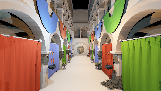
\includegraphics[width=\linewidth]{screen-effects/taa.png}}{32 · 两个采样位置的平均颜色}
\caption{遮蔽和反射两图导出第四个数，分别表示可见程度和反射射线的命中标记。右图取 TAA 的 RGB。静止相机下，回放中两次采样各占一半，可见表面的平均历史权重为 0.5。}
\end{figure}

环境遮蔽（GTAO）会沿几个屏幕方向寻找可见地平线。正常半径下，可见表面的平均可见程度为 0.899；把半径缩到 0.0001 个场景单位，平均升到 0.9997，说明原来变暗的部分来自附近的遮挡。随机屏幕反射的粗糙度取 0.08，36.34\% 的可见像素找到了画面中的反射点。固定种子重复计算得到相同颜色；粗糙度改为 0.65 后，反射方向的分布随之改变。命中率本身不能说明反射方向正确，画外和被挡住的表面也不会出现在屏幕输入里。

TAA 的对照把八个略有偏移的采样位置分别画出，保存各自的直接光，再离线取平均。相对于这份平均图，第八个单帧的均方误差为 0.001698。修正静止镜头的历史取样后，TAA 第八帧与八次取样平均仅差浮点舍入误差（$1.11\times10^{-16}$）。把镜头平移一个单位，全图约 41.0\% 的像素继续使用历史；手动重置后，全图历史权重降为零。上图捕获的是预先画过一帧、随后在未偏移镜头下再次使用历史的短序列。

\readings{八帧对照与固定种子复现见 \path{tests/ScreenEffectsTests.cpp}、
\path{tests/screen_effects_report.py} 和 \path{output/screen-effects/metrics.json}。每项算法各有一个计算着色器，文件在 \path{Renderer/ScreenSpace/Shaders/}。}

\clearpage
\section{49 盏灯怎样分配给画面}
在一条有 49 盏灯的走廊里，先把画面切成 $16\times16$ 像素的小块，再按深度分成 16 层。事件 47 为每个小空间建立灯表；事件 58 只计算表中灯的贡献。这组历史对照用四单位半径、纯漫反射和无遮挡来单测筛选。正式场景读取各点光源的半径，再检查阴影与材质高光。

\begin{figure}[H]\centering
\panelimage{.45\linewidth}{
\includegraphics[width=\linewidth]{screen-effects/clustered-mask.png}}{每个像素要检查的灯数，白色代表 49}
\hfill\panelimage{.45\linewidth}{
\includegraphics[width=\linewidth]{screen-effects/clustered.png}}{事件 58 写出的线性颜色，经曝光显示}
\caption{同一帧的两次导出。全图有 1,056 个小空间，每个用两个 32 位整数记录 49 盏灯。回放中有 627 个空间记录了编号 33 至 49 中至少一盏。}
\end{figure}

逐像素检查时，14,501 个可见像素平均访问 18.11 盏灯。用 CPU 在每个像素遍历全部 49 盏灯，两种方式得到的 RGB 最大绝对差为 $1.20\times10^{-7}$。把灯清空，输出也降为零。这里直接测到了候选数下降；要判断整帧能省多少时间，还需在相同 GPU 上对照逐灯着色与分簇两条路径，包括建立灯表的成本。

{\noindent\smalltable\begin{tabularx}{\linewidth}{@{}Xrrrr@{}}\toprule
GPU 执行内容 & 事件 & 工作组数 & 中位数（ms） & 范围（ms）\\\midrule
\screenTimingRows\bottomrule\end{tabularx}\par}

捕获来自 RTX 5070 Ti Laptop GPU，Debug/x64，分辨率 $161\times91$，右边和底边都有不完整的工作组。上表先预热一次，再以 RenderDoc 1.47 读取九轮执行时间。回放中的遮蔽、反射、分簇颜色都与独立 GPU 读回逐值相同。要比较桌面分辨率的开销，下一次应扩大视口、保持相机与灯不变，并单独测纹理读取与同步等待。

\readings{原始帧及其复现说明见 \path{output/profiling/screen-effects/}。}
